\section{Credit Invariant}

Each node $x$ has at least $\mu(x)$ tokens on its account.

%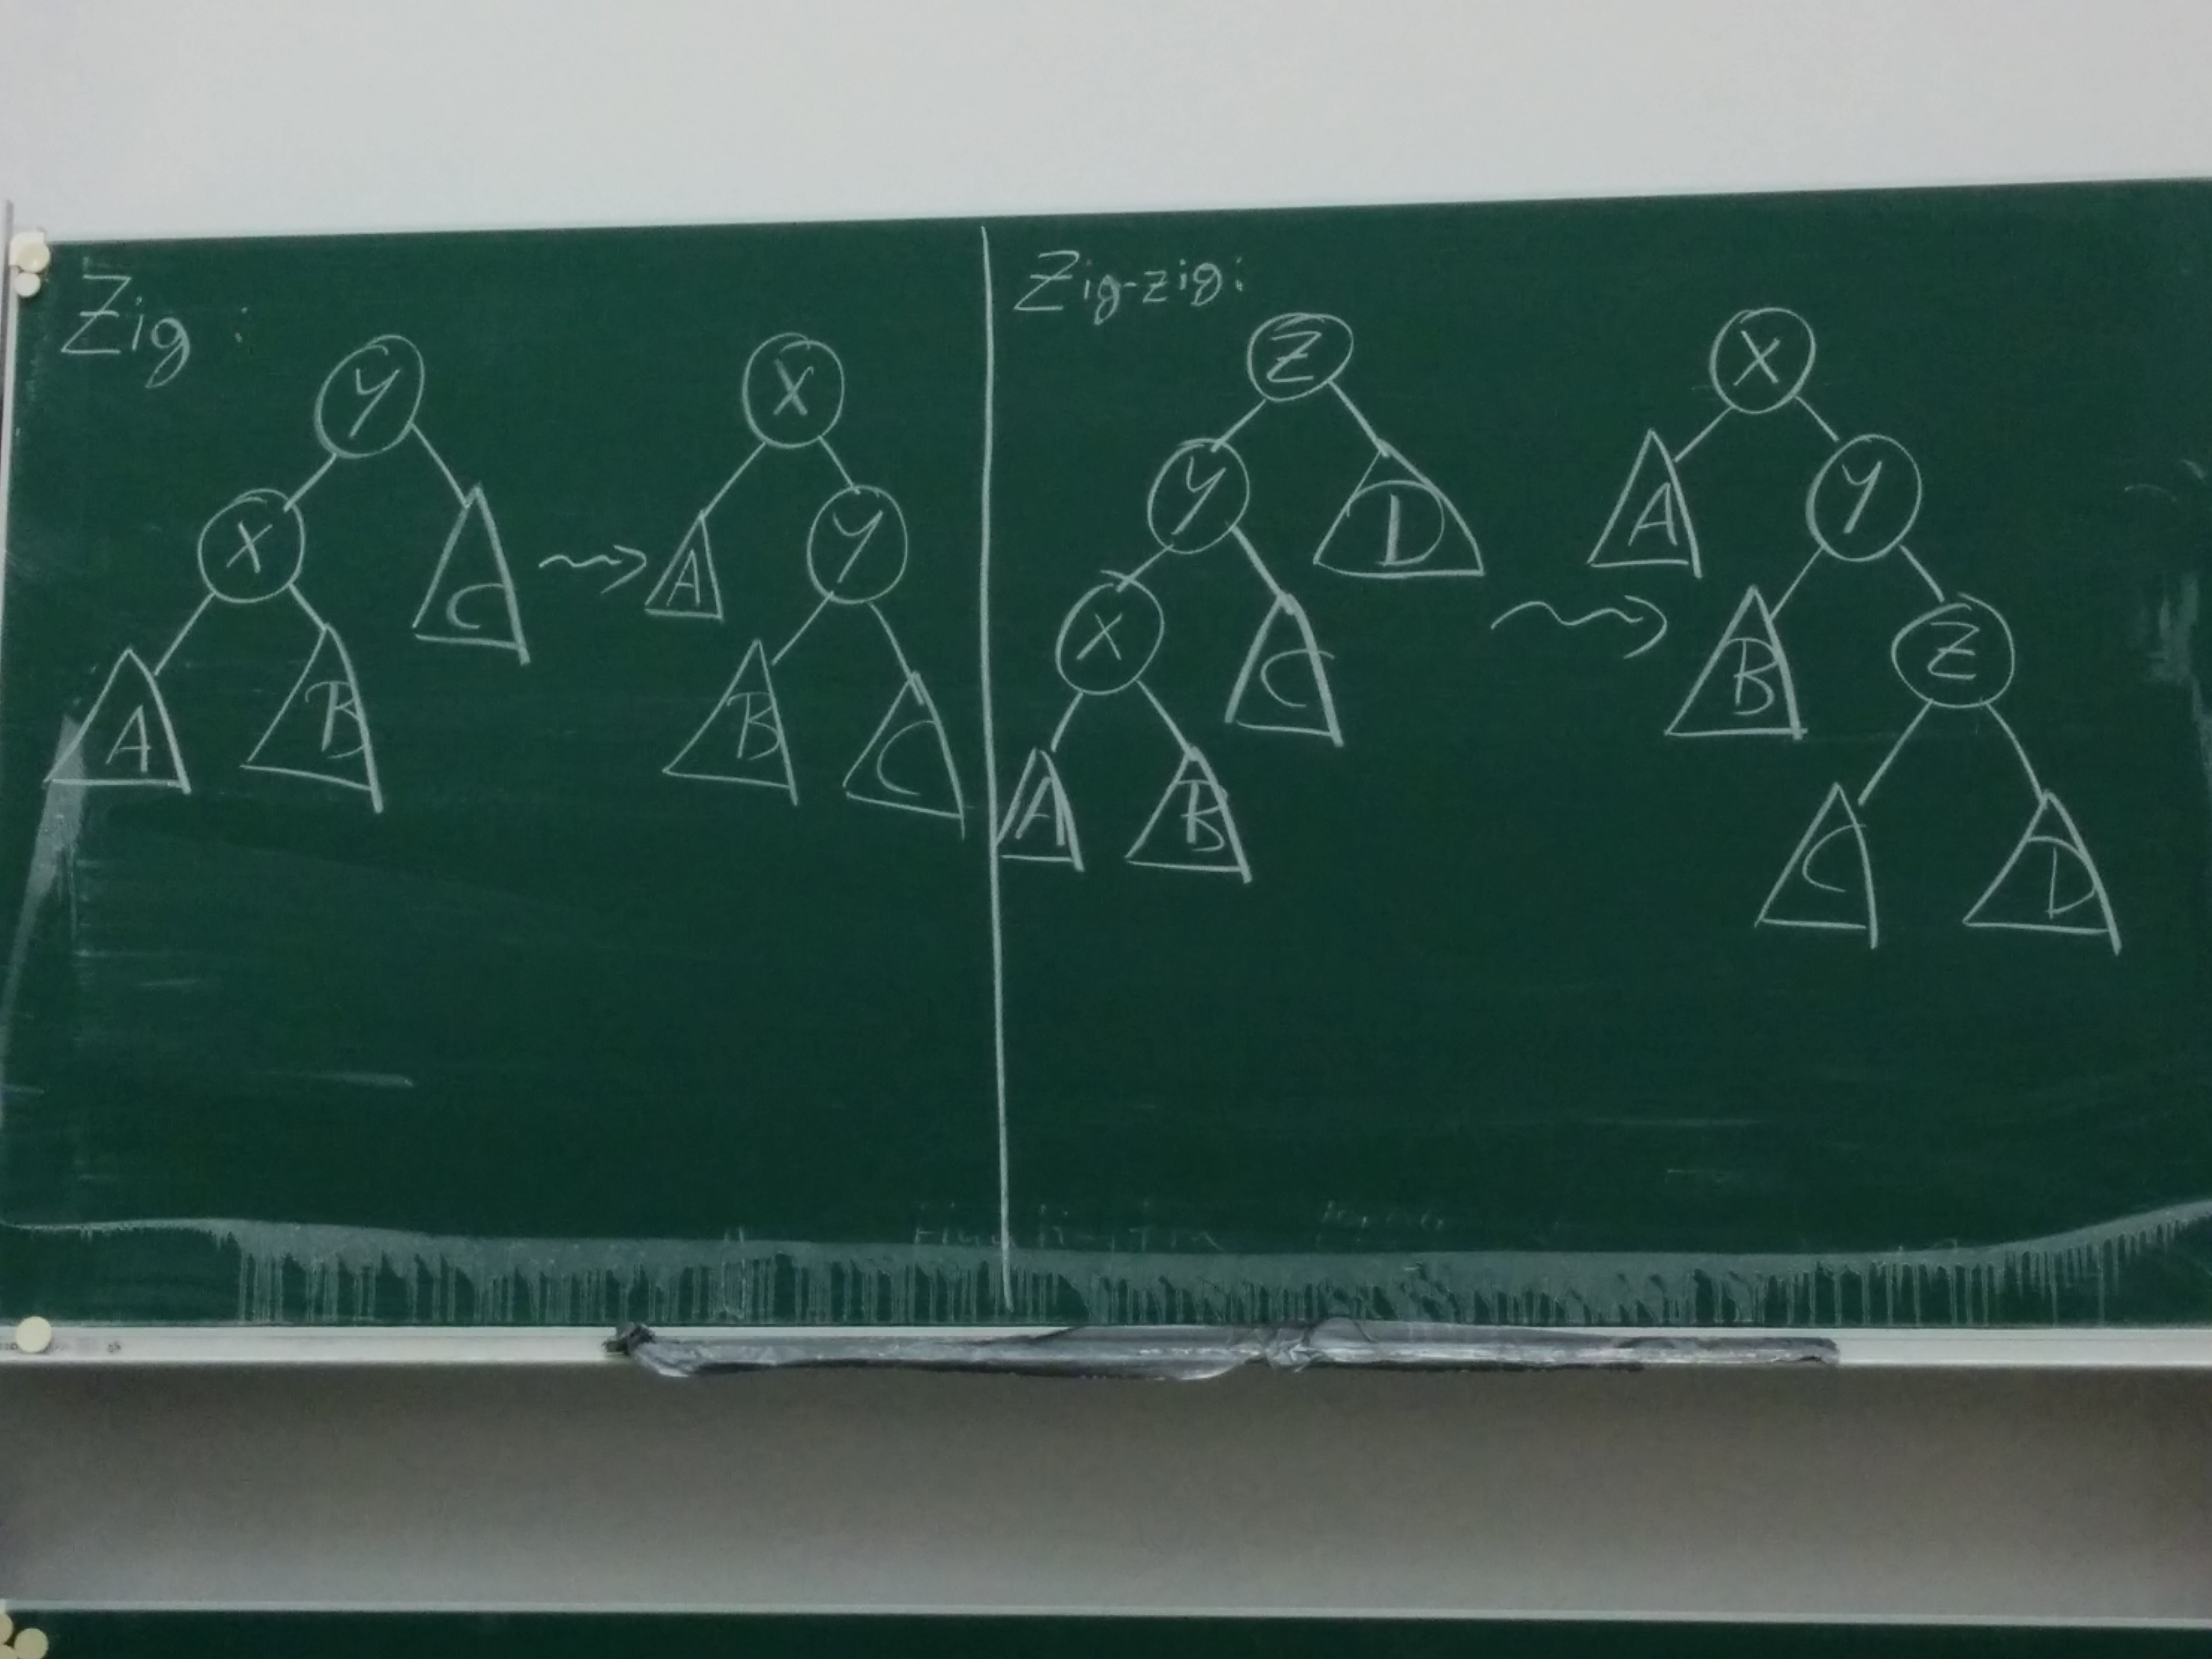
\includegraphics[width=430px]{tree1.jpg}

%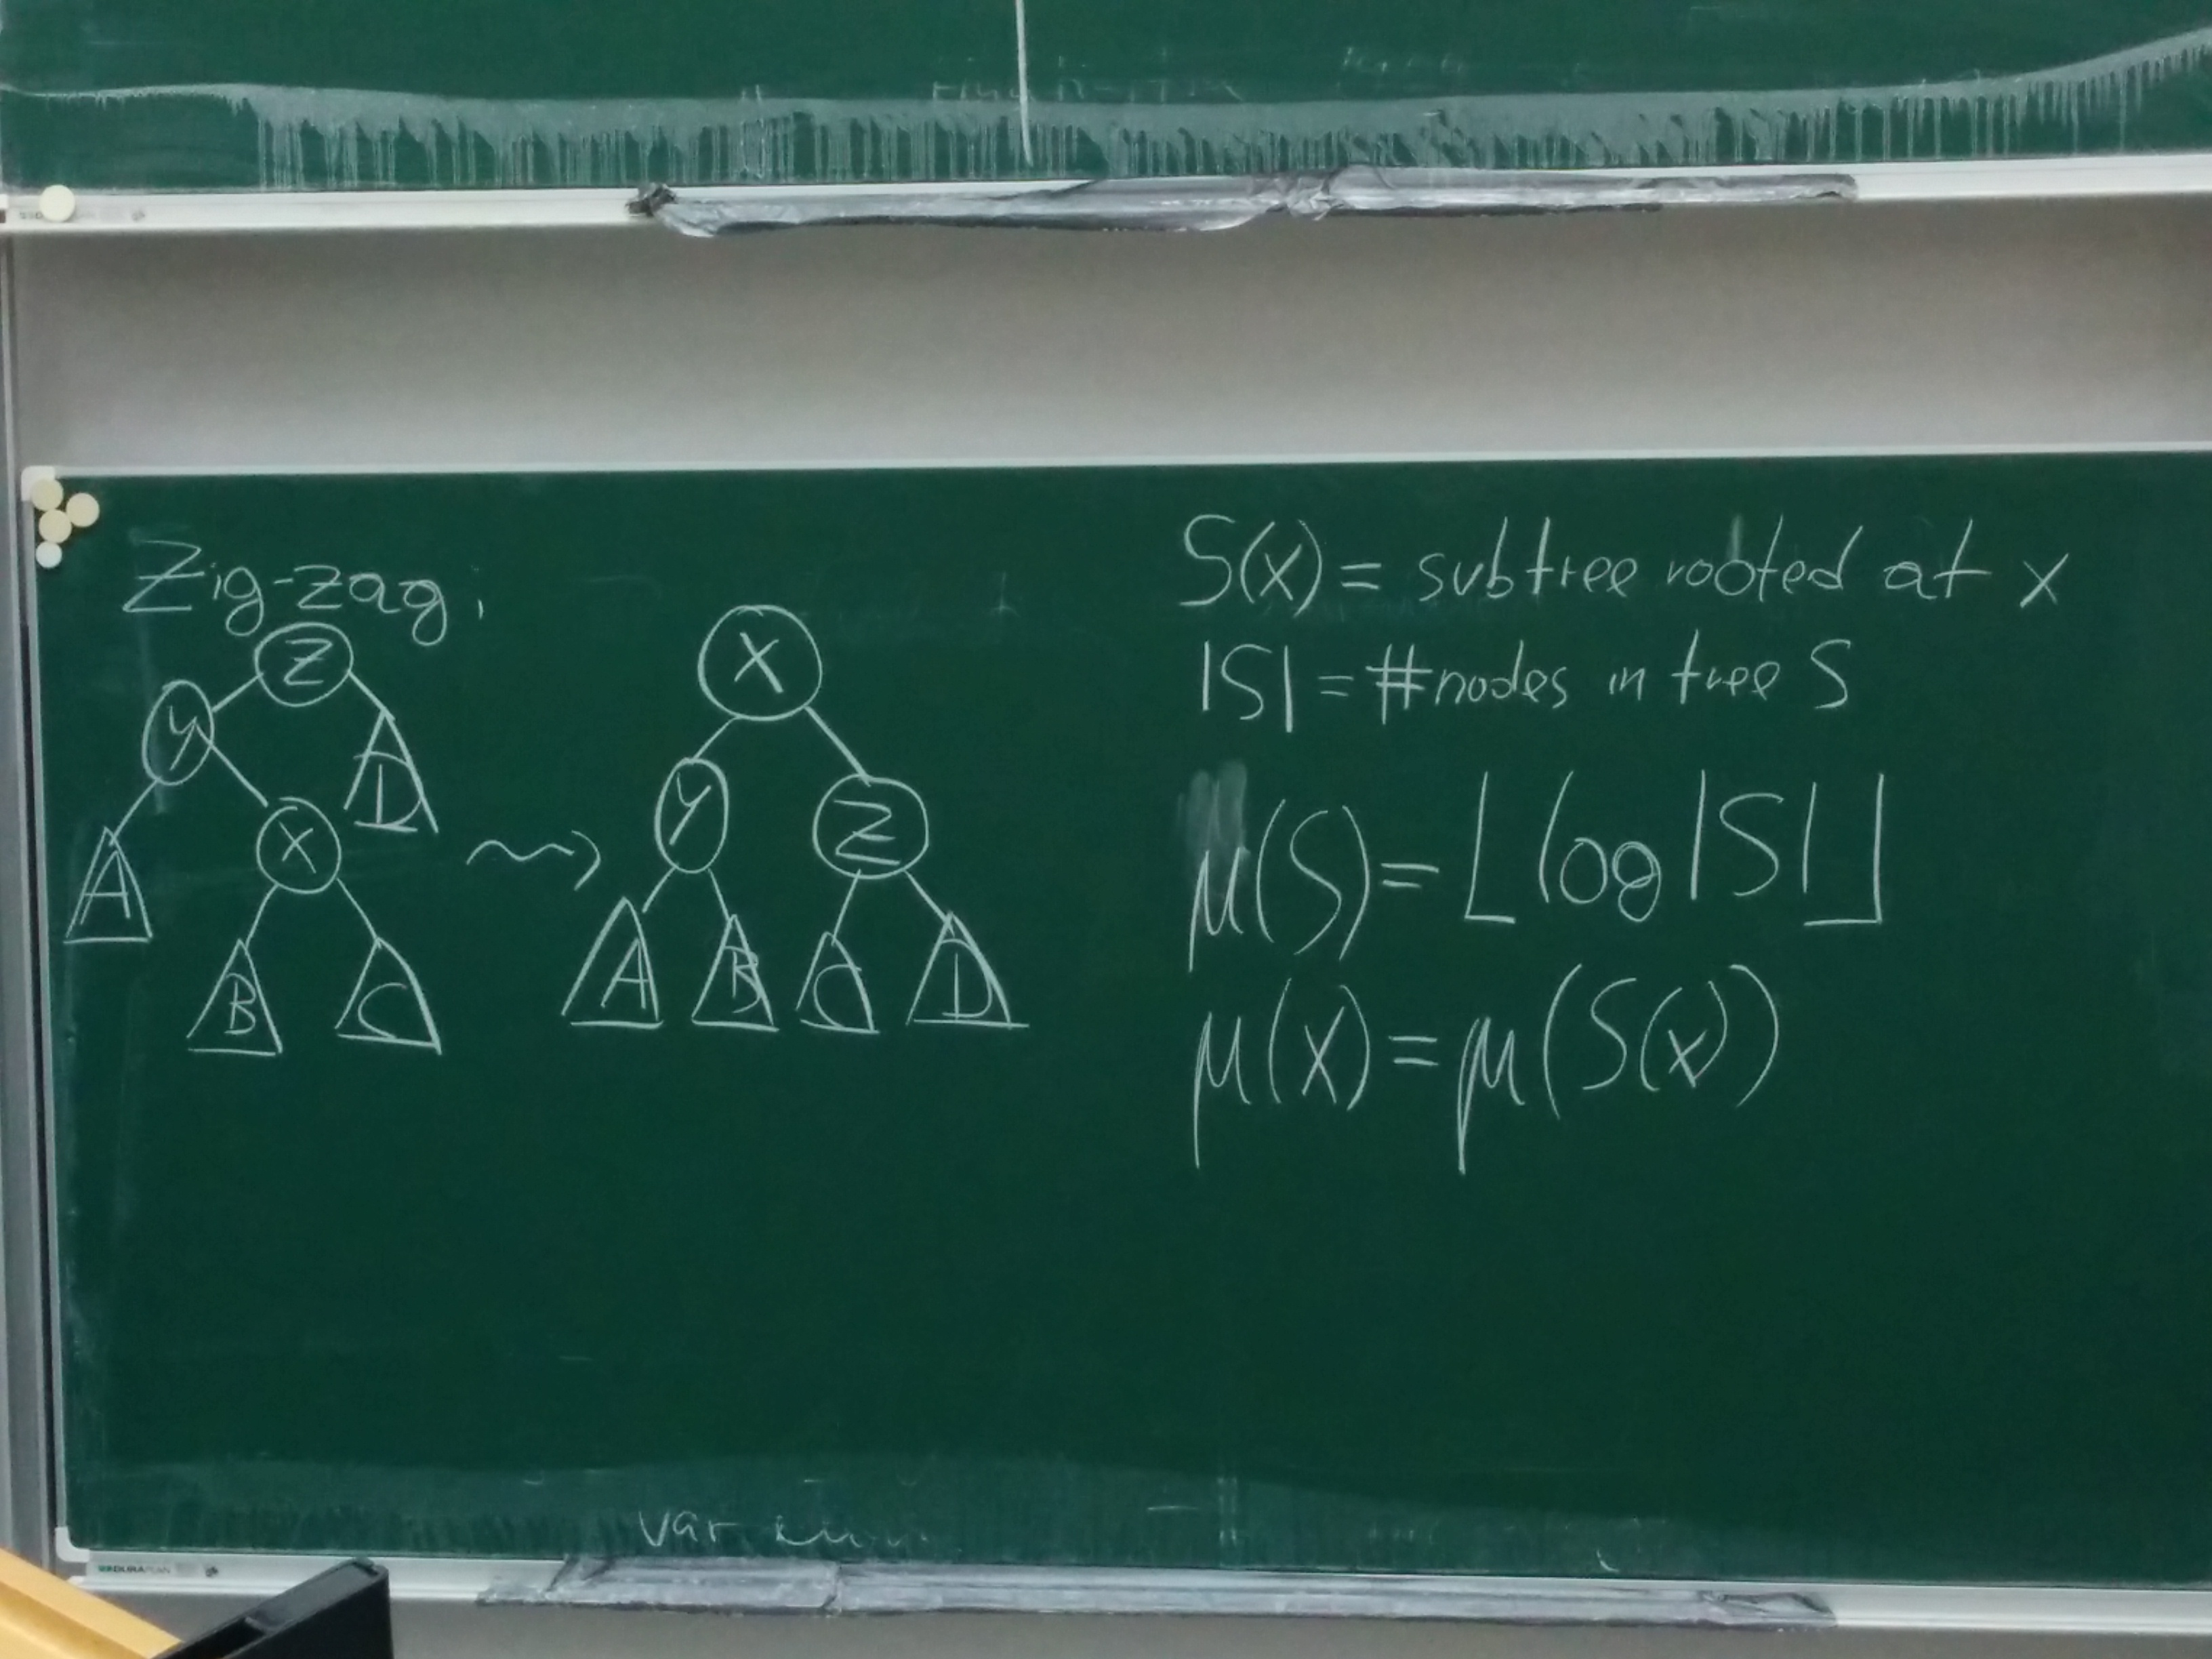
\includegraphics[width=430px]{tree2.jpg}

\begin{mylemma}
Let $x$ be the node that becomes root after a splay operation on tree $T$. We need to spent at most

$$3(\mu(T)-\mu(x)) + 1$$

tokens to pay for all steps and maintain the credit invariant.
\end{mylemma}
\begin{proof}
The cost of finding $x$ is proportional to the cost of rotating $x$ to the root, so we can concentrate on the latter.

For a fixed rotation, let $\mu$ and $\mu'$ denote the weight of a node before and after the rotation. We show:

\begin{enumerate}
\item In a zig-case, we need to pay at most $3(\mu'(x) - \mu(x)) + 1$ tokens.
\item In zig-zig or zig-zag case, we need to pay at most $3(\mu'(x)-\mu(X))$ tokens.
\end{enumerate}

$$[3(\mu'(x)-\mu(x))+3(\mu''(x)-\mu'(x)) + \ldots = 3(\mu(T)-\mu(x))+1] \text{ (telescoping sum)}$$

\paragraph{Proof of (i):} We have that $\mu(y) = \mu'(x)$, and $\mu'(y) \le \mu'(x)$. We have to pay:

\begin{align*}
\underbrace{(\mu'(x) - \mu(x))}_\text{credit inv. for $x$} \quad + \quad \underbrace{(\mu'(y)-\mu(y))}_\text{credit inv. for $y$} \quad + \quad \underbrace{1}_\text{for paying the rotation}  
& \le \mu'(x) -\mu(x) + 1 \\
& \le 3(\mu'(x) - \mu(x)) + 1
\end{align*}

\paragraph{Proof of (ii):} Consider a zig-zag. We need

$$C = \mu'(x) - \mu(x) + \mu'(y) - \mu(y) + \mu'(z) - \mu(z) + 1$$

tokens. Since $\mu'(x) - \mu(z)$, this simplifies to:

\begin{align*}
C & \le \mu'(y) - \mu(x) + \mu'(z) - \mu(y) + 1 \\
& \le \mu'(x) - \mu(x) + \mu'(x) - \mu(x) + 1 \\
& = 2(\mu'(x) - \mu(x)) + 1
\end{align*}

If $\mu(x) - \mu(x) > 0$, this is at most $3(\mu'(x) - \mu(x))$ and we are done. What if $\mu(x) = \mu(x)$? We show that $\mu(x)=\mu(x)$ implies that $C\le 0$, so we have to spend $0 \le 3(\mu'(x)-\mu(x)$.

By contradiction, assume $\mu'(x)=\mu(x)$ and $C\ge 1$. That means $\mu'(x)=\mu(x)$ and $(\mu'(x)+\mu'(y)+\mu'(z) \ge \mu(x)+\mu(y)+\mu(z)$.

Since $\mu(x)=\mu'(x)=\mu(z)$, we have that $\mu(y) = \mu(x) = \mu(z)$. So, the inequality simplifies to

$$\mu'(y) + \mu'(z) \ge 2\mu'(x),$$

which implies $\mu'(x) = \mu'(y) = \mu'(z) = \mu(x) = \mu(y) = \mu(z)$.

Consider $a = |S(x)|$ before rotating, and $b = |S(z)|$ after rotating.

Then $\underbrace{\lfloor \log a \rfloor}_{=\mu(x)} = \underbrace{\lfloor\log a + b + 1\rfloor}_{=\mu'(x)} = \underbrace{\lfloor \log b \rfloor}_{=\mu'(z)}$

For $a \le b$, $\mu'(x) = \lfloor \log a + b + a \rfloor \ge \lfloor \log 2a \rfloor \ge 1 + \lfloor \log a \rfloor > \lfloor \log a \rfloor$.

So $C \le 0$.
\end{proof}

\begin{mytheorem}
For an initially empty splay tree, a sequence of $m$ insertions/removals/searches with $n$ inserts costs $O(m \log n)$.
\end{mytheorem}
\begin{proof}
Every splay step pays $O(\log n)$ tokens to perform all operations. When inserting a node, we have to put $\log n$ tokens on its account for the credit invariant.
\end{proof}

\section{Heaps}

\begin{itemize}
\item Sorted sequences with restricted access patterns.
\item Elements have keys (priorities) as usual
\end{itemize}

A \emph{non-addressable priority queue} $Q$ supports:
\begin{itemize}
\item ${insert}(e, Q)$
\item ${min}(Q)$: return element with smallest key
\item ${delete\_min}(Q)$: remove smallest element
\item ${build}(e_1, \ldots, e_n)$: creates a priorirty queue with elements $e_1, \ldots, e_n$
\end{itemize}

A handle $h$ is a pointer to an element stored in $A$.
An \emph{addressable priorirty queue} $Q$ supports:
\begin{itemize}
\item ${insert}(e, Q)$: returns a handle to inserted element
\item ${remove}(h, Q)$: remove the element pointed by $h$
\item ${min}(Q)$
\item ${delete\_min}(Q)$
\item ${build}(e_1, \ldots, e_n)$
\item ${decrease\_key}(h, k, Q)$: replaces the key of $h$ with $k$ (must be smaller than old key)
\item ${union}(Q_1, Q_2)$: merges the priority queues $Q_1$ and $Q_2$
\end{itemize}

\subsection{Binary Heaps}

\begin{itemize}
\item It is a maximally balanced binary tree
\item Last level is left-aligned
\item One element per node
\item Heap-ordered: key at node $v$ is smaller than all keys in descendants of $v$
\item Can be stored as an array
\end{itemize}

\begin{lstlisting}[mathescape]
${insert}(e, Q)$:
    put $e$ at next free position in node $v$
    sift_up(v)
    
${sift\_up}(v)$:
    if $v$ is root, return
    $w \gets {parent}(v)$
    if ${key}(v) > {key}(w)$, return
    else
        swap elements of $v$ and $w$
        ${sift\_up}(w)$
\end{lstlisting}

\begin{lstlisting}[mathescape]
${delete\_min}(Q)$:
    swap elements of root and last element in order
    delete last element
    ${sift\_down}({root})$

${sift\_down}(v)$:
    if $v$ is leaf, return
    $w \gets$ smallest child of $v$
    if ${key}(v) < {key}(w)$, return
    else
        swap contents of $v$ and $w$
        ${sift\_down}(w)$
\end{lstlisting}

\paragraph{Build: } Let $e_1, \ldots, e_n$ be the elements of the heap. Put the elements in any order and call ${heapify}({root})$.
\begin{lstlisting}[mathescape]
${heapify}(v)$:
    if $v$ has left child $w$:
        ${heapify}(w)$
    if $v$ has right child $w'$:
        ${heapify}(w')$
    ${sift\_down}(v)$
\end{lstlisting}

\paragraph{Cost: } A ${sift\_down}$ on level $i$ costs not more than $\log n -i$ steps. The total cost is given by:

\begin{align*}
\sum_{i = 0}^{\lfloor \log n \rfloor} 2^i (\log n - i) \\
& = \sum_{j = 0}^{\lfloor \log n \rfloor} 2^i (\log n - j) j \\
& = n \cdot \underbrace{\sum_{j = 0}^{\lfloor \log n \rfloor} \frac{1}{2^j} \cdot j}_{\le 2} \\
& = O(n)
\end{align*}

\begin{align*}
\sum_{j=0}^\infty \frac{j}{2^j} = \sum_{j \ge 1} \frac{j}{2^j} & = \sum_{j \ge 1} \frac{1}{2^j} + \sum_{j \ge 2} \frac{1}{2^j} + \sum_{j \ge 3} \frac{1}{2^j} + \ldots  \\
& = \sum_{j \ge 1} \frac{1}{2^j} + \frac{1}{2} \sum_{j \ge 2} \frac{1}{2^{j-1}} + \frac{1}{4} \sum_{j \ge 3} \frac{1}{2^{j-2}} + \ldots \\
& = \sum_{j \ge 1} \frac{1}{2^j} + \frac{1}{2} \sum_{j \ge 1} \frac{1}{2^j} + \frac{1}{4} \sum_{j \ge 1} \frac{1}{2^j} + \ldots \\
& = \underbrace{\sum_{j \ge 1} \frac{1}{2^j}}_{=1} \left ( 1 + \frac{1}{2} + \frac{1}{4} + \ldots \right ) \\
& \le 2
\end{align*}




